% Options for packages loaded elsewhere
\PassOptionsToPackage{unicode}{hyperref}
\PassOptionsToPackage{hyphens}{url}
\documentclass[
  12pt,
]{article}
\usepackage{xcolor}
\usepackage[left=3cm,right=3cm,top=3cm,bottom=3cm]{geometry}
\usepackage{amsmath,amssymb}
\setcounter{secnumdepth}{-\maxdimen} % remove section numbering
\usepackage{iftex}
\ifPDFTeX
  \usepackage[T1]{fontenc}
  \usepackage[utf8]{inputenc}
  \usepackage{textcomp} % provide euro and other symbols
\else % if luatex or xetex
  \usepackage{unicode-math} % this also loads fontspec
  \defaultfontfeatures{Scale=MatchLowercase}
  \defaultfontfeatures[\rmfamily]{Ligatures=TeX,Scale=1}
\fi
\usepackage{lmodern}
\ifPDFTeX\else
  % xetex/luatex font selection
\fi
% Use upquote if available, for straight quotes in verbatim environments
\IfFileExists{upquote.sty}{\usepackage{upquote}}{}
\IfFileExists{microtype.sty}{% use microtype if available
  \usepackage[]{microtype}
  \UseMicrotypeSet[protrusion]{basicmath} % disable protrusion for tt fonts
}{}
\makeatletter
\@ifundefined{KOMAClassName}{% if non-KOMA class
  \IfFileExists{parskip.sty}{%
    \usepackage{parskip}
  }{% else
    \setlength{\parindent}{0pt}
    \setlength{\parskip}{6pt plus 2pt minus 1pt}}
}{% if KOMA class
  \KOMAoptions{parskip=half}}
\makeatother
\usepackage{color}
\usepackage{fancyvrb}
\newcommand{\VerbBar}{|}
\newcommand{\VERB}{\Verb[commandchars=\\\{\}]}
\DefineVerbatimEnvironment{Highlighting}{Verbatim}{commandchars=\\\{\}}
% Add ',fontsize=\small' for more characters per line
\usepackage{framed}
\definecolor{shadecolor}{RGB}{248,248,248}
\newenvironment{Shaded}{\begin{snugshade}}{\end{snugshade}}
\newcommand{\AlertTok}[1]{\textcolor[rgb]{0.94,0.16,0.16}{#1}}
\newcommand{\AnnotationTok}[1]{\textcolor[rgb]{0.56,0.35,0.01}{\textbf{\textit{#1}}}}
\newcommand{\AttributeTok}[1]{\textcolor[rgb]{0.13,0.29,0.53}{#1}}
\newcommand{\BaseNTok}[1]{\textcolor[rgb]{0.00,0.00,0.81}{#1}}
\newcommand{\BuiltInTok}[1]{#1}
\newcommand{\CharTok}[1]{\textcolor[rgb]{0.31,0.60,0.02}{#1}}
\newcommand{\CommentTok}[1]{\textcolor[rgb]{0.56,0.35,0.01}{\textit{#1}}}
\newcommand{\CommentVarTok}[1]{\textcolor[rgb]{0.56,0.35,0.01}{\textbf{\textit{#1}}}}
\newcommand{\ConstantTok}[1]{\textcolor[rgb]{0.56,0.35,0.01}{#1}}
\newcommand{\ControlFlowTok}[1]{\textcolor[rgb]{0.13,0.29,0.53}{\textbf{#1}}}
\newcommand{\DataTypeTok}[1]{\textcolor[rgb]{0.13,0.29,0.53}{#1}}
\newcommand{\DecValTok}[1]{\textcolor[rgb]{0.00,0.00,0.81}{#1}}
\newcommand{\DocumentationTok}[1]{\textcolor[rgb]{0.56,0.35,0.01}{\textbf{\textit{#1}}}}
\newcommand{\ErrorTok}[1]{\textcolor[rgb]{0.64,0.00,0.00}{\textbf{#1}}}
\newcommand{\ExtensionTok}[1]{#1}
\newcommand{\FloatTok}[1]{\textcolor[rgb]{0.00,0.00,0.81}{#1}}
\newcommand{\FunctionTok}[1]{\textcolor[rgb]{0.13,0.29,0.53}{\textbf{#1}}}
\newcommand{\ImportTok}[1]{#1}
\newcommand{\InformationTok}[1]{\textcolor[rgb]{0.56,0.35,0.01}{\textbf{\textit{#1}}}}
\newcommand{\KeywordTok}[1]{\textcolor[rgb]{0.13,0.29,0.53}{\textbf{#1}}}
\newcommand{\NormalTok}[1]{#1}
\newcommand{\OperatorTok}[1]{\textcolor[rgb]{0.81,0.36,0.00}{\textbf{#1}}}
\newcommand{\OtherTok}[1]{\textcolor[rgb]{0.56,0.35,0.01}{#1}}
\newcommand{\PreprocessorTok}[1]{\textcolor[rgb]{0.56,0.35,0.01}{\textit{#1}}}
\newcommand{\RegionMarkerTok}[1]{#1}
\newcommand{\SpecialCharTok}[1]{\textcolor[rgb]{0.81,0.36,0.00}{\textbf{#1}}}
\newcommand{\SpecialStringTok}[1]{\textcolor[rgb]{0.31,0.60,0.02}{#1}}
\newcommand{\StringTok}[1]{\textcolor[rgb]{0.31,0.60,0.02}{#1}}
\newcommand{\VariableTok}[1]{\textcolor[rgb]{0.00,0.00,0.00}{#1}}
\newcommand{\VerbatimStringTok}[1]{\textcolor[rgb]{0.31,0.60,0.02}{#1}}
\newcommand{\WarningTok}[1]{\textcolor[rgb]{0.56,0.35,0.01}{\textbf{\textit{#1}}}}
\usepackage{longtable,booktabs,array}
\usepackage{calc} % for calculating minipage widths
% Correct order of tables after \paragraph or \subparagraph
\usepackage{etoolbox}
\makeatletter
\patchcmd\longtable{\par}{\if@noskipsec\mbox{}\fi\par}{}{}
\makeatother
% Allow footnotes in longtable head/foot
\IfFileExists{footnotehyper.sty}{\usepackage{footnotehyper}}{\usepackage{footnote}}
\makesavenoteenv{longtable}
\usepackage{graphicx}
\makeatletter
\newsavebox\pandoc@box
\newcommand*\pandocbounded[1]{% scales image to fit in text height/width
  \sbox\pandoc@box{#1}%
  \Gscale@div\@tempa{\textheight}{\dimexpr\ht\pandoc@box+\dp\pandoc@box\relax}%
  \Gscale@div\@tempb{\linewidth}{\wd\pandoc@box}%
  \ifdim\@tempb\p@<\@tempa\p@\let\@tempa\@tempb\fi% select the smaller of both
  \ifdim\@tempa\p@<\p@\scalebox{\@tempa}{\usebox\pandoc@box}%
  \else\usebox{\pandoc@box}%
  \fi%
}
% Set default figure placement to htbp
\def\fps@figure{htbp}
\makeatother
\setlength{\emergencystretch}{3em} % prevent overfull lines
\providecommand{\tightlist}{%
  \setlength{\itemsep}{0pt}\setlength{\parskip}{0pt}}
\usepackage{fontspec}
\usepackage{indentfirst}
\usepackage{setspace}
\usepackage{fvextra}
\fvset{breaklines=true,breakanywhere=true}
\setmainfont{Times New Roman}
\setlength{\parindent}{1.18cm}
\setstretch{1.5}
\usepackage{bookmark}
\IfFileExists{xurl.sty}{\usepackage{xurl}}{} % add URL line breaks if available
\urlstyle{same}
\hypersetup{
  hidelinks,
  pdfcreator={LaTeX via pandoc}}

\author{}
\date{\vspace{-2.5em}}

\begin{document}

\begin{center}

{\Large \textbf{ANALISIS DATA PEMBANGUNAN WILAYAH}}

{\Large \textbf{MENGGUNAKAN R}}

\vspace{0.5cm}

\textbf{Disusun Oleh:}

\vspace{0.5cm}

\begin{tabular}{p{8cm}p{3cm}}
Muhamad Akbar Zainuri & J0403251008\
Zalfa Nazla Azkiya & J0403251037\
Diaz Ramaananta Harahap & J0403251048\
Dede Risma Komalasari & J0403251049\
Nashira Salima Firmansyah & J0403251056\
Fahrizal Azis & J0403251151\
\end{tabular}

\vspace{0.5cm}


\includegraphics[width=3.5cm]{../gambar/Logo_IPB.png}

\vspace{0.5cm}

\large{\textbf{MATA KULIAH PROBABILITAS & STATISTIKA}}

\large{\textbf{PROGRAM STUDI TEKNOLOGI REKAYASA PERANGKAT LUNAK}}

\large{\textbf{SEKOLAH VOKASI}}

\large{\textbf{INSTITUT PERTANIAN BOGOR}}

\large{\textbf{BOGOR}}

\large{\textbf{2026}}

\end{center}

bf\{INSTITUT PERTANIAN BOGOR\}\}

\large\{\textbf{BOGOR}\}

\large\{\textbf{2026}\}

\textbackslash end\{center\}

\thispagestyle{empty}
\newpage

\begin{center}
{
\bfseries

```
\vfill

\Large

DAFTAR ISI

```

}

\end{center}

\begin{flushleft}
BAB I \dotfill 1\
\hspace*{0.5cm}1.1 Latar Belakang \dotfill 1\
\hspace*{0.5cm}1.2 Tujuan \dotfill 1\[0.3cm]

BAB II \dotfill 2\
\hspace*{0.5cm}2.1 Dataset \dotfill 2\
\hspace*{0.5cm}2.2 Tools Yang Digunakan \dotfill 2\
\hspace*{0.5cm}2.3 Metode Analisis \dotfill 2\[0.3cm]

BAB III \dotfill 3\
\hspace*{0.5cm}3.1 Statistika Deskriptif \dotfill 3\
\hspace*{0.5cm}3.2 Missing Value \dotfill 3\
\hspace*{0.5cm}3.3 Outlier \dotfill 3\
\hspace*{0.5cm}3.4 Visualisasi \dotfill 3\
\hspace*{0.5cm}3.5 Distribusi Data \dotfill 3\
\hspace*{0.5cm}3.6 Korelasi \dotfill 3\
\hspace*{0.5cm}3.7 Interpretasi \dotfill 3\[0.3cm]

BAB IV \dotfill 4\
\hspace*{0.5cm}4.1 Kesimpulan Utama \dotfill 4\
\hspace*{0.5cm}4.2 Insight \dotfill 4\
\hspace*{0.5cm}4.3 Saran \dotfill 4\[0.3cm]

LAMPIRAN \dotfill 5\
\hspace*{0.5cm}5.1 Script R \dotfill 5\
\hspace*{0.5cm}5.2 Output Tambahan \dotfill 5\
\end{flushleft}

BAB III \dotfill 3\\
\hspace*{0.5cm}3.1 Statistika Deskriptif \dotfill 3\\
\hspace*{0.5cm}3.2 Missing Value \dotfill 3\\
\hspace*{0.5cm}3.3 Outlier \dotfill 3\\
\hspace*{0.5cm}3.4 Visualisasi \dotfill 3\\
\hspace*{0.5cm}3.5 Distribusi Data \dotfill 3\\
\hspace*{0.5cm}3.6 Korelasi \dotfill 3\\
\hspace*{0.5cm}3.7 Interpretasi \dotfill 3{[}0.3cm{]}

BAB IV \dotfill 4\\
\hspace*{0.5cm}4.1 Kesimpulan Utama \dotfill 4\\
\hspace*{0.5cm}4.2 Insight \dotfill 4\\
\hspace*{0.5cm}4.3 Saran \dotfill 4{[}0.3cm{]}

LAMPIRAN \dotfill 5\\
\hspace*{0.5cm}5.1 Script R \dotfill 5\\
\hspace*{0.5cm}5.2 Output Tambahan \dotfill 5\\
\textbackslash end\{flushleft\}

\thispagestyle{empty}

\newpage

\begin{center}
{
\bfseries

```
\vfill

\Large

BAB I

PENDAHULUAN

```

}
\end{center}

\subsection{\texorpdfstring{\normalsize 1.1 \hspace {0,5cm} Latar
Belakang}{1.1  Latar Belakang}}\label{latar-belakang}

\vspace{-0.5cm}

Pembangunan wilayah adalah sebuah proses yang bertujuan untuk
meningkatkan kesejahteraan masyarakat. Untuk mengetahui bagaimana suatu
pembangunan wilayah di suatu daerah berhasil diperlukan indikator yang
dapat menggambarkan keadaan masyarakat di wilayah tersebut dengan jelas,
seperti angka kemiskinan, pengangguran, Produk Domestik Regional Bruto
(PDRB), serta indeks pembangunan Manusia (IPM).

Oleh karena itu, diperlukan analisis data untuk mengolah informasi yang
ada agar dapat memberikan gambaran tentang kondisi pembangunan di suatu
wilayah. Berdasarkan kebutuhan tersebut, projek ini bertujuan untuk
menganalisis data pembangunan wilayah di seluruh Indonesia dengan
mengimplementasikan bahasa pemrograman R. Melalui projek akhir ini,
mahasiswa diharapkan dapat meningkatkan keterampilan mereka dalam
mengolah, menganalisis, dan menginterpretasikan data terkait pembangunan
daerah dengan memanfaatkan bahasa pemrograman R.

\subsection{\texorpdfstring{\normalsize 1.2 \hspace {0,5cm}
Tujuan}{1.2  Tujuan}}\label{tujuan}

\vspace{-0.5cm}

Proyek ini bertujuan untuk menganalisis data mengenai pembangunan
wilayah di Indonesia dengan memanfaatkan bahasa pemrograman R. Analisis
dilakukan untuk mengenali ciri-ciri data, memahami hubungan di antara
indikator pembangunan, serta mengungkap faktor-faktor yang memengaruhi
tingkat perkembangan suatu daerah. Di samping itu, proyek ini bertujuan
untuk mengaplikasikan konsep statistika dan analisis data dalam
menyelesaikan masalah yang ada serta menyajikan hasil analisis dengan
cara yang terstruktur dan informatif.

\setcounter{page}{1}
\newpage

\begin{center}
{
\bfseries

```
\vfill

\Large

BAB II

METODOLOGI

```

}
\end{center}

\subsection{\texorpdfstring{\normalsize 2.1 \hspace {0,5cm}
Dataset}{2.1  Dataset}}\label{dataset}

\vspace{-0.5cm}

Dataset adalah kumpulan data terstruktur yang digunakan untuk berbagai
keperluan, seperti analisis, penelitian, atau pengolahan informasi
lainnya. Di dalam sebuah dataset, terdapat sejumlah variabel yang
disusun dalam bentuk tabel. Setiap kolom mewakili atribut tertentu,
sementara setiap baris menggambarkan entitas atau observasi yang
berbeda. Dataset menjadi komponen penting dalam pengolahan data,
membantu menghasilkan informasi yang lebih bermakna dan bermanfaat.

Data yang digunakan dalam analisis ini adalah dataset skor pembangunan
wilayah tingkat Kabupaten/Kota di Indonesia. Secara keseluruhan, dataset
ini mencakup observasi 2.500 baris kabupaten/kota dengan 13 kolom
variabel, yang berada dalam rentang waktu lima tahun, yaitu dari tahun
2020 hingga 2024. Berikut adalah rincian variabel-variabel yang telah
dikelompokkan menjadi beberapa kategori:

\begin{enumerate}
\def\labelenumi{\arabic{enumi}.}
\tightlist
\item
  Variabel Identitas Data : wilayah, provinsi, dan tahun.
\item
  Variabel Ekonomi : pdrb\_perkapita, kemiskinan, dan pengangguran.
\item
  Variabel Pembangunan Manusia : ipm, harapan\_hidup,
  rata\_lama\_sekolah.
\item
  Variabel Infrastruktur : akses\_internet, jalan\_baik, air\_bersih.
\item
  Variabel Metadata : catatan\_data.
\end{enumerate}

Dataset pembangunan wilayah tersebut berbentuk dokumen .csv. Dokumen ini
bisa diunduh melalui
\url{https://pembangunanwilayahmissingoutlier.tiiny.site} untuk melihat
dataset secara keseluruhan.

\subsection{\texorpdfstring{\normalsize 2.2 \hspace {0,5cm} Tools Yang
Digunakan}{2.2  Tools Yang Digunakan}}\label{tools-yang-digunakan}

\vspace{-0.5cm}

Dalam melakukan analisis data ini, digunakan perangkat lunak Rstudio dan
library ggplot2 untuk menghasilkan informasi yang terstruktur dan akurat
tentang pembangunan wilayah di Indonesia. Berikut adalah rincian tools
yang digunakan:

\begin{enumerate}
\def\labelenumi{\arabic{enumi}.}
\tightlist
\item
  \textbf{Dataset format .csv:} Digunakan sebagai format penyimpanan
  data mentah yang menjadi objek utama analisis.
\item
  \textbf{Bahasa Pemrograman R:} R digunakan sebagai bahasa pemrograman
  utama untuk komputasi statistik dan analisis data. Bahasa ini dipilih
  karena memiliki kemampuan yang kuat dalam melakukan manipulasi data,
  serta menyediakan berbagai paket statistik yang mumpuni untuk
  melakukan analisis deskriptif maupun inferensial pada dataset.
\item
  \textbf{RStudio:} RStudio digunakan sebagai \emph{Integrated
  Development Environment} (IDE) atau lingkungan pengembangan
  terintegrasi untuk menulis dan mengeksekusi kode R. RStudio
  mempermudah manajemen proyek, pemantauan variabel, penanganan error
  melalui antarmuka yang interaktif, serta mendukung penyusunan laporan
  menggunakan R Markdown.
\item
  \textbf{Library ggplot2:} Library ggplot2 digunakan untuk memenuhi
  kebutuhan visualisasi data. Library ini memungkinkan pembuatan grafik
  secara modular. Di dalam proyek ini, ggplot2 digunakan untuk
  menyajikan tren indikator pembangunan, mengidentifikasi sebaran data,
  serta memberikan visualisasi perbandingan kondisi antarwilayah secara
  informatif.
\end{enumerate}

\subsection{\texorpdfstring{\normalsize 2.3 \hspace {0,5cm} Metode
Analisis}{2.3  Metode Analisis}}\label{metode-analisis}

\vspace{-0.5cm}

Analisis data dilakukan menggunakan bahasa pemrograman R untuk
memperoleh gambaran mengenai kondisi pembangunan wilayah di Indonesia.
Tahapan analisis yang dilakukan adalah sebagai berikut:

\begin{enumerate}
\def\labelenumi{\arabic{enumi}.}
\tightlist
\item
  \textbf{Pengumpulan Data:} Data yang digunakan merupakan data
  indikator pembangunan wilayah yang mencakup beberapa variabel
  pdrb\_perkapita, kemiskinan, pengangguran, IPM, akses\_internet, dll).
\item
  \textbf{Analisis Statistik Deskriptif:} Analisis statistik deskriptif
  dilakukan untuk menggambarkan karakteristik data melalui nilai
  minimum, nilai maksimum, rata-rata, median, standar deviasi, dan
  lain-lain.
\item
  \textbf{Analisis Missing Value:} Missing value dianalisis dengan
  menghitung jumlah dan persentase data yang hilang pada seiap variabel.
  Hasil analisis digunakan untuk menentukan metode penanganan yang
  sesuai.
\item
  \textbf{Analisis Outlier:} Deteksi outlier dilakukan menggunakan
  metode Interquartile Range (IQR). Suatu data dikatakan sebagai outlier
  apabila berada di luar batas.
\item
  \textbf{Visualisasi Data:} Visualisasi dilakukan untuk mempermudah
  interpretasi data menggunakan histogram, boxplot, scatter plot, dan
  heatmap korelasi.
\item
  \textbf{Analisis Korelasi:} Analisis korelasi digunakan untuk
  mengetahui hubungan antar indikator pembangunan wilayah. Kolerasi
  dihitung menggunakan koefisien korelasi pearson dengan rentang nilai
  −1 ≤ r ≤ 1. Nilai korelasi yang mendekati 1 menunjukkan hubungan
  positif yang kuat, sedangkan nilai yang mendekati -1 menunjukkan
  hubungan negatif yang kuat.
\end{enumerate}

\setcounter{page}{2}
\newpage

\begin{center}
{
\bfseries

```
\vfill

\Large

BAB III

HASIL DAN PEMBAHASAN

```

}
\end{center}

\subsection{\texorpdfstring{\normalsize 3.1 \hspace {0,5cm} Statistika
Deskriptif}{3.1  Statistika Deskriptif}}\label{statistika-deskriptif}

\vspace{-0.5cm}

Statistika deskriptif merupakan metode statistik yang digunakan untuk
meringkas dan menggambarkan karakteristik utama dari suatu kumpulan data
secara numerik. Analisis ini bertujuan untuk memberikan gambaran awal
mengenai kondisi data pembangunan wilayah, khususnya terkait ukuran
pemusatan data seperti mean dan median serta ukuran penyebaran data
seperti standar deviasi, varians, dan rentang nilai.

Pada penelitian ini, analisis statistika deskriptif dilakukan terhadap
seluruh variabel numerik pada dataset pembangunan wilayah menggunakan
beberapa fungsi dalam bahasa pemrograman R seperti \textit{summary()},
\textit{mean()}, \textit{median()}, \textit{sd()}, \textit{var()}, dan
\textit{quantile()}.

\vspace{-0.5cm}

\begin{center}
\textbf{Tabel 3.1 Hasil Statistika Deskriptif}

\begin{tabular}{|l|c|c|c|}
\hline
\textbf{Variabel} & \textbf{Mean} & \textbf{SD} & \textbf{Keterangan} \
\hline
pdrb_perkapita & Tinggi & Paling besar & Penyebaran sangat tinggi \
\hline
kemiskinan & 13,72 & Cukup besar & Terdapat variasi data \
\hline
pengangguran & 8 & Besar & Indikasi data ekstrem \
\hline
ipm & 69--70 & Relatif kecil & Distribusi stabil \
\hline
harapan_hidup & 69 tahun & Relatif kecil & Distribusi stabil \
\hline
rata_lama_sekolah & 9,5 tahun & Relatif kecil & Distribusi stabil \
\hline
\end{tabular}

\end{center}

harapan\_hidup \& 69 tahun \& Relatif kecil \& Distribusi stabil\\
\hline rata\_lama\_sekolah \& 9,5 tahun \& Relatif kecil \& Distribusi
stabil\\
\hline \textbackslash end\{tabular\}

\textbackslash end\{center\}

Berdasarkan hasil analisis, variabel \textit{pdrb_perkapita} memiliki
nilai rata-rata tertinggi dibandingkan variabel lainnya. Selain itu,
variabel tersebut juga mempunyai standar deviasi terbesar yang
menunjukkan bahwa terdapat perbedaan tingkat pendapatan yang cukup besar
antar wilayah di Indonesia.

Variabel \textit{kemiskinan} dan \textit{pengangguran} juga menunjukkan
penyebaran data yang cukup besar. Hal ini terlihat dari rentang nilai
minimum dan maksimum yang jauh berbeda. Pada variabel pengangguran,
nilai maksimum bahkan jauh di atas rata-ratanya sehingga mengindikasikan
adanya beberapa data ekstrem.

Sementara itu, variabel seperti \textit{ipm}, \textit{harapan_hidup},
dan \textit{rata_lama_sekolah} memiliki nilai mean dan median yang
relatif berdekatan. Kondisi tersebut menunjukkan bahwa distribusi data
pada variabel pembangunan manusia cenderung lebih stabil dan tidak
terlalu menyebar.

Perbedaan mean dan median yang cukup jauh pada beberapa variabel ekonomi
memberikan indikasi awal bahwa data kemungkinan tidak berdistribusi
normal serta terdapat outlier pada beberapa wilayah. Oleh karena itu,
analisis lanjutan mengenai missing value dan outlier perlu dilakukan
pada tahap berikutnya.

\subsection{\texorpdfstring{\normalsize 3.2 \hspace {0,5cm} Missing
Value}{3.2  Missing Value}}\label{missing-value}

\vspace{-0.5cm}

\textit{Missing value}, atau data yang hilang, terjadi ketika salah satu
kolom atau atribut dalam dataset tidak memiliki nilai. Hal Ini bisa
disebabkan oleh kesalahan pencatatan, keterbatasan teknis selama proses
pengumpulan data, atau kondisi tertentu di mana data memang tidak
tersedia. Misalnya, dalam analisis data pembangunan ini, jika data IPM
hilang, sulit menyimpulkan tingkat pembangunan wilayah secara
keseluruhan

Pada penelitian ini, penanganan dilakukan terhadap baris data yang
memiliki \textit{missing value} dalam dataset pembangunan wilayah
menggunakan bahasa pemrograman R, yang dimulai dengan mengukur terlebih
dahulu seberapa besar pengaruhnya dalam data.

\vspace{6cm}

\begin{center}
\textbf{Tabel 3.2 Hasil Analisis \textit{Missing Value}}

\begin{tabular}{|c|c|c|}
\hline
\textbf{Variabel} & \textbf{Missing Value} & \textbf{Persentase} \
\hline
pdrb_perkapita & 25 & 1% \
\hline
kemiskinan & 24 & 0.96% \
\hline
pengangguaran & 25 & 1% \
\hline
IPM & 25 & 1% \
\hline
akses_internet & 25 & 1% \
\hline
jalan_baik & 25 & 1% \
\hline
\multicolumn{2}{|l|}{\textbf{Rata-Rata Persentase}} & 0.45% \
\hline
\end{tabular}

\end{center}

\textbackslash end\{center\}

Berdasarkan hasil analisis, ditemukan \textit{missing value} pada
beberapa variabel seperti \textit{pdrb_perkapita}, \textit{kemiskinan},
\textit{pengangguran}, \textit{IPM}, \textit{akses_internet}, dan
\textit{jalan_baik}. Keberadaan \textit{missing value} ini dapat
mempengaruhi hasil analisis statistik, salah satu contohnya adalah
mengurangi jumlah observasi yang dapat di analisis.

Data yang memiliki nilai kosong tidak dapat digunakan secara langsung
dalam berbagai metode statistik. Akibatnya, jumlah data yang tersedia
untuk analisis menjadi berkurang sehingga informasi yang diperoleh
menjadi kurang lengkap.

Untuk metode penanganan \textit{missing value} itu sendiri, yang kami
gunakan adalah penghapusan. Metode ini dipilih karena proporsi data yang
hilang pada setiap variabel relatif kecil yaitu 1\% dari total
observasi, dimana tidak menyebabkan berkurangnya representativitas data
secara signifikan, sehingga dampaknya terhadap analisis diperkirakan
sangat kecil.

Alasan lainnya adalah, metode ini sederhana dan sangat efektif jika
jumlah \textit{missing value} kecil, misalnya 1-2\% dari data. Namun,
jika jumlah data yang hilang mencapai 30\% atau lebih, metode ini
beresiko mengurangi informasi penting dan tidak disarankan.

\subsection{\texorpdfstring{\normalsize 3.3 \hspace {0,5cm}
Outlier}{3.3  Outlier}}\label{outlier}

\vspace{-0.5cm}

\textit{Outlier} adalah nilai yang berbeda secara signifikan dari
sebagian besar data lainnya, sering kali muncul karena kesalahan
pengukuran, variasi alami, atau anomali yang tidak terduga.
\textit{Outlier} dapat berdampak negatif pada analisis, seperti
menggeser rata-rata. Oleh karena itu, deteksi dan penanganan
\textit{outlier} menjadi langkah penting yang harus dilakukan.

Pada penelitian ini, dataset pembangunan wilayah memiliki outlier pada
sejumlah variabel, yaitu \textit{pdrb_perkapita}, \textit{kemiskinan},
dan \textit{pengangguran}. Berikut penjabaran seberapa banyak outlier
yang dimiliki setiap variebal tersebut.

\vspace{-0.5cm}

\begin{center}
\textbf{Tabel 3.3 Hasil Analisis \textit{Outlier}}

\begin{tabular}{|c|c|}
\hline
\textbf{Variabel} & \textbf{Jumlah Outlier} \
\hline
pdrb_perkapita & 5 \
\hline
kemiskinan & 5 \
\hline
pengangguran & 5 \
\hline
\end{tabular}
\end{center}

pengangguran \& 5\\
\hline \textbackslash end\{tabular\} \textbackslash end\{center\}

\begin{center}
\textbf{Gambar 3.1 Boxplot Outlier}
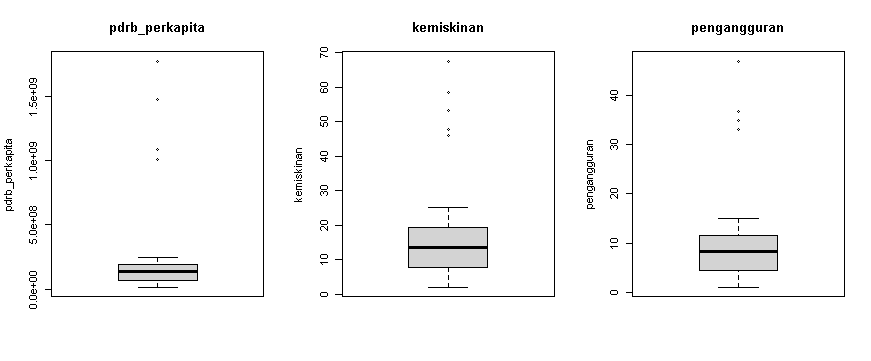
\includegraphics[width=15cm]{../gambar/boxplot_outlier.png}
\end{center}

\vspace{-2cm}

\begin{center}
\textbf{Tabel 3.4 Nilai-Nilai \textit{Outlier} yang Terdeteksi}

\begin{tabular}{|c|c|c|}
\hline
\textbf{pdrb_perkapita} & \textbf{kemiskinan} & \textbf{pengangguran} \
\hline
1.012.449.971 & 45,95 & 33,19 \
\hline
1.087.231.959 & 47,69 & 34,90 \
\hline
1.472.419.961 & 53,50 & 36,68 \
\hline
1.474.832.345 & 58,41 & 36,74 \
\hline
1.774.545.027 & 67,53 & 47,04 \
\hline
\end{tabular}
\end{center}

1.474.832.345 \& 58,41 \& 36,74\\
\hline
1.774.545.027 \& 67,53 \& 47,04\\
\hline \textbackslash end\{tabular\} \textbackslash end\{center\}

Dalam analisis ini, metode deteksi \textit{outlier} yang kami gunakan
adalah \textbf{IQR}. Metode ini mengidentifikasi \textit{outlier} dengan
menghitung rentang antara kuartil pertama (Q1) dan kuartil ketiga (Q3).
Nilai yang berada diluar rentang {[}Q1 - 1.5 x IQR, Q3 + 1.5 x IQR{]}
dianggap sebagai \textit{outlier}.

Nilai \textit{outlier} juga memiliki dampak besar terhadap analisis
statistik, salah satu contohnya adalah, \textit{outlier} dapat menarik
ukuran pemusatan data ke arah nilai ekstrem. Berikut tabel dampak nilai
\textit{outlier} yang sudah di analisis.

\vspace{-0.5cm}

\begin{center}
\textbf{Tabel 3.5 Dampak \textit{Outlier} terhadap Nilai Rata-Rata}

\begin{tabular}{|c|c|c|c|}
\hline
\textbf{Variabel} & \textbf{Mean Sebelum Penghapusan} & \textbf{Mean Setelah Penghapusan} & \textbf{Selisih} \
\hline
pdrb_perkapita & 135.650.462 & 133.163.326 & 2.487.136 \
\hline
kemiskinan & 13.72 & 13.64 & 0.08 \
\hline
pengangguran & 8.05 & 7.99 & 0.06 \
\hline
\end{tabular}
\end{center}

pengangguran \& 8.05 \& 7.99 \& 0.06\\
\hline \textbackslash end\{tabular\} \textbackslash end\{center\}

Variabel \textit{pdrb_perkapita} mengalami perubahan rata-rata terbesar
setelah \textit{outlier} dihapus, yaitu sebesar 2.487.136. Ini
menunjukkan bahwa keberadaan beberapa daerah dengan nilai
\textit{pdrb_perkapita} yang sangat tinggi memberikan pengaruh yang
cukup besar terhadap nilai rata-rata keseluruhan. Sementara itu,
variabel kemiskinan dan pengangguran hanya mengalami perubahan rata-rata
yang relatif kecil, sehingga pengaruh \textit{outlier} terhadap kedua
variabel tersebut tidak sebesar pada variabel \textit{pdrb_perkapita}.

\subsection{\texorpdfstring{\normalsize 3.4 \hspace {0,5cm}
Visualisasi}{3.4  Visualisasi}}\label{visualisasi}

\vspace{-0.5cm}

\begin{center}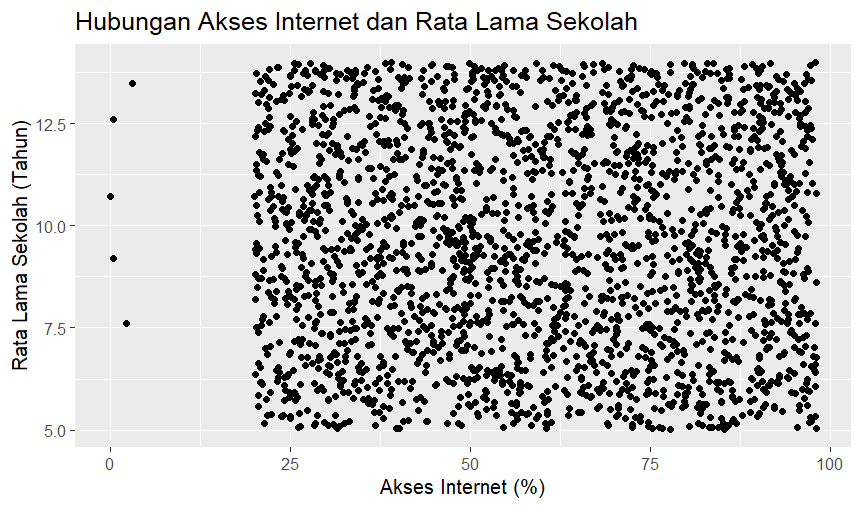
\includegraphics[width=0.85\linewidth]{../gambar/hubAksesInternet&rataLamaSekolah} \end{center}

\begin{center}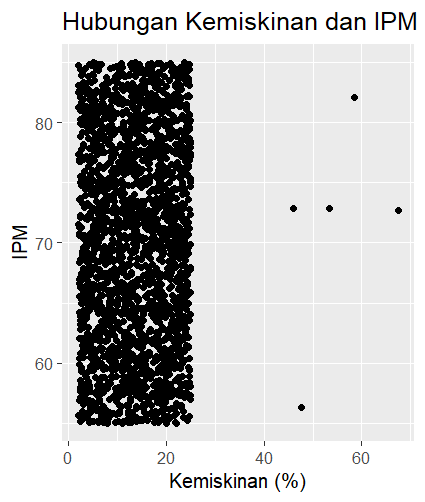
\includegraphics[width=0.85\linewidth]{../gambar/hubungankemiskinandgIPM} \end{center}

Berdasarkan visualisasi data yang dilakukan, terdapat beberapa temuan
penting mengenai hubungan antar variabel makroekonomi dan sosial.
Pertama, analisis diagram pencar (\textit{scatter plot}) antara variabel
tingkat akses internet terhadap rata-rata lama sekolah menunjukkan
sebaran data yang membentuk pola persegi panjang yang sangat padat.
Mayoritas titik observasi terkonsentrasi secara merata pada rentang
persentase akses internet antara 20\% hingga 100\%, dengan rata-rata
lama sekolah berkisar antara 5 hingga 14 tahun. Secara visual, tidak
terlihat adanya tren linier naik ataupun turun yang cukup kuat dan
signifikan. Namun, terdapat fenomena menarik di sisi kiri ekstrem grafik
(mendekati 0\% akses internet), di mana ditemukan sekitar 5 titik data
terisolasi yang berjejer secara vertikal.

Sementara itu, visualisasi hubungan antara tingkat kemiskinan dan Indeks
Pembangunan Manusia (IPM) menunjukkan pemisahan kelompok data
(\textit{clustering}) yang sangat kontras. Kelompok pertama membentuk
klaster vertikal yang sangat padat di sebelah kiri grafik pada rentang
tingkat kemiskinan rendah hingga menengah (antara 2\% hingga 25\%),
dengan sebaran nilai IPM yang bervariasi lebar dari skala 55 hingga 85.
Sebaliknya, kelompok kedua berada di sisi kanan grafik yang diisi oleh 5
titik data pencilan (\textit{outliers}) yang tersebar renggang pada
tingkat kemiskinan ekstrem antara 45\% hingga 70\%.

\vspace{0.2cm}

\subsection{\texorpdfstring{\normalsize 3.5 \hspace {0,5cm} Distribusi
Data}{3.5  Distribusi Data}}\label{distribusi-data}

\vspace{-0.5cm}

\begin{longtable}[]{@{}lll@{}}
\caption{Hasil Uji Normalitas Shapiro-Wilk}\tabularnewline
\toprule\noalign{}
Variabel & P-Value & Kesimpulan \\
\midrule\noalign{}
\endfirsthead
\toprule\noalign{}
Variabel & P-Value & Kesimpulan \\
\midrule\noalign{}
\endhead
\bottomrule\noalign{}
\endlastfoot
IPM & 2.379285e-25 & Tidak Berdistribusi Normal \\
Kemiskinan & 2.377348e-29 & Tidak Berdistribusi Normal \\
Akses Internet & 6.137887e-26 & Tidak Berdistribusi Normal \\
\end{longtable}

Analisis distribusi data dilakukan untuk mengetahui karakteristik
sebaran data serta menilai apakah data mengikuti distribusi normal atau
tidak. Pada penelitian ini digunakan uji normalitas Shapiro-Wilk
terhadap variabel IPM, kemiskinan, dan akses internet dengan tingkat
signifikansi sebesar 5\% (\(\alpha = 0,05\)). Berdasarkan Tabel 3.7,
ketiga variabel memiliki nilai p-value yang jauh lebih kecil dari 0,05
sehingga disimpulkan bahwa data \textbf{tidak berdistribusi normal}.

Berdasarkan grafik \textit{boxplot}, variabel PDRB per kapita memiliki
distribusi yang sangat menjulur. Kotak interkuartil dan garis median
menumpuk sangat rendah di bagian bawah mendekati nilai \(0.0\), namun di
atas garis batas \textit{whisker} atas ditemukan beberapa titik pencilan
(\textit{outliers}) ekstrem yang berada pada kisaran nilai
\(1.0 \times 10^9\) hingga mendekati \(1.8 \times 10^9\).

Untuk variabel IPM, grafik histogram menunjukkan bentuk distribusi yang
relatif merata pada rentang nilai 55 hingga 85, dengan frekuensi yang
konsisten. Modus berada pada kisaran nilai IPM 70--73. Karakteristik ini
didukung oleh grafik \textit{Normal Q-Q Plot} yang membentuk pola
menyerupai huruf S (\textit{S-shaped curve}). Data cenderung mengikuti
garis referensi linier hanya pada bagian tengah (kuantil teoritis -1
hingga 1), sedangkan pada kedua ujungnya melengkung menjauhi garis
referensi, mengindikasikan adanya deviasi distribusi.

Terakhir, distribusi tingkat kemiskinan memiliki rata-rata sebesar
13,72\% dengan pola yang menumpuk padat di sebelah kiri
(\textit{right-skewed}). Berdasarkan perhitungan probabilitas empiris,
peluang wilayah memiliki tingkat kemiskinan di atas rata-rata adalah
sekitar \textbf{45\%}. Selanjutnya, peluang suatu wilayah memiliki nilai
IPM \textgreater{} 75 diperoleh sebesar \textbf{30\%}, sedangkan untuk
IPM \textless{} 75 mencapai \textbf{72\%}. Perhitungan persentil ke-95
menunjukkan nilai IPM berada pada angka \textbf{83,9}, yang berarti
hanya sekitar 5\% wilayah di Indonesia yang memiliki kualifikasi IPM
sangat tinggi. Deviasi distribusi ini diperkuat oleh grafik
\textit{Normal Q-Q Plot} kemiskinan, di mana mayoritas data melengkung
mendatar di bagian bawah sebelum melonjak tajam secara diskrit di ujung
kanan atas akibat adanya pencilan ekstrem.

\vspace{0.2cm}

\subsection{\texorpdfstring{\normalsize 3.6 \hspace {0,5cm}
Korelasi}{3.6  Korelasi}}\label{korelasi}

\vspace{-0.5cm}

Analisis korelasi merupakan metode statistik yang digunakan untuk
mengetahui hubungan antar variabel dalam suatu dataset. Pada penelitian
ini, analisis korelasi dilakukan menggunakan metode \textit{Pearson}
untuk mengukur kekuatan serta arah hubungan linear antar variabel
pembangunan wilayah.

Variabel yang dianalisis meliputi \textit{pdrb_perkapita},
\textit{kemiskinan}, \textit{pengangguran}, \textit{ipm},
\textit{harapan_hidup}, \textit{rata_lama_sekolah}, dan
\textit{akses_internet}. Hasil analisis korelasi ditampilkan dalam
bentuk ringkasan berikut.

\vspace{-0.5cm}

\begin{center}
\textbf{Tabel 3.8 Hasil Analisis Korelasi}

\begin{tabular}{|c|c|c|c|}
\hline
\textbf{Variabel 1} & \textbf{Variabel 2} & \textbf{Nilai Korelasi} & \textbf{Keterangan} \
\hline
pdrb_perkapita & kemiskinan & -0,0048 & Sangat lemah (negatif) \
\hline
pengangguran & pdrb_perkapita & -0,0323 & Sangat lemah (negatif) \
\hline
ipm & pdrb_perkapita & 0,0111 & Sangat lemah (positif) \
\hline
harapan_hidup & pdrb_perkapita & 0,0125 & Sangat lemah (positif) \
\hline
akses_internet & kemiskinan & -0,0309 & Sangat lemah (negatif) \
\hline
akses_internet & ipm & 0,0020 & Sangat lemah (positif) \
\hline
\end{tabular}
\end{center}

p \& pdrb\_perkapita \& 0,0125 \& Sangat lemah (positif)\\
\hline akses\_internet \& kemiskinan \& -0,0309 \& Sangat lemah
(negatif)\\
\hline akses\_internet \& ipm \& 0,0020 \& Sangat lemah (positif)\\
\hline \textbackslash end\{tabular\} \textbackslash end\{center\}

Berdasarkan hasil analisis, seluruh nilai korelasi berada sangat dekat
dengan nol, yaitu dalam rentang sekitar -0,03 hingga 0,01. Hal ini
menunjukkan bahwa hubungan linear antar variabel dalam dataset
pembangunan wilayah sangat lemah.

Tidak adanya korelasi yang kuat mengindikasikan bahwa variabel-variabel
tersebut tidak memiliki hubungan linear yang signifikan dan kemungkinan
dipengaruhi oleh faktor lain di luar model yang digunakan.

\subsection{\texorpdfstring{\normalsize 3.7 \hspace {0,5cm}
Interpretasi}{3.7  Interpretasi}}\label{interpretasi}

\setcounter{page}{3}
\newpage

\begin{center}
{
\bfseries

```
\vfill

\Large

BAB IV

KESIMPULAN

```

}
\end{center}

\subsection{\texorpdfstring{\normalsize 4.1 \hspace {0,5cm} Kesimpulan
Utama}{4.1  Kesimpulan Utama}}\label{kesimpulan-utama}

\vspace{-0.5cm}

Berdasarkan hasil analisis data pembangunan wilayah menggunakan bahasa
pemrograman R, dapat disimpulkan bahwa dataset memiliki kualitas yang
baik dengan tingkat \emph{missing value} yang sangat rendah, yaitu
sekitar 0,45\% dari keseluruhan data. Penanganan \emph{missing value}
dilakukan dengan metode penghapusan karena proporsinya relatif kecil dan
tidak memengaruhi representativitas data secara signifikan.

Analisis statistika deskriptif menunjukkan bahwa variabel ekonomi
memiliki tingkat variasi yang lebih tinggi dibandingkan variabel
pembangunan manusia. Selain itu, analisis \emph{outlier} menunjukkan
adanya beberapa data ekstrem pada variabel PDRB per kapita, kemiskinan,
dan pengangguran.

Hasil analisis korelasi menunjukkan bahwa hubungan antar indikator
pembangunan dalam dataset cenderung lemah dan tidak signifikan secara
statistik. Dengan demikian, pembangunan wilayah merupakan fenomena yang
kompleks dan dipengaruhi oleh berbagai faktor yang saling berkaitan.

\subsection{\texorpdfstring{\normalsize 4.2 \hspace {0,5cm}
Insight}{4.2  Insight}}\label{insight}

\vspace{-0.5cm}

\begin{enumerate}
\def\labelenumi{\arabic{enumi}.}
\tightlist
\item
  Ketimpangan ekonomi antar wilayah masih terlihat dari adanya outlier
  pada variabel PDRB per kapita.
\item
  Variabel pembangunan manusia seperti IPM, harapan hidup, dan rata-rata
  lama sekolah memiliki distribusi yang relatif stabil.
\item
  Hubungan antar indikator pembangunan pada dataset tidak menunjukkan
  pola linear yang kuat.
\item
  Analisis pembangunan wilayah memerlukan pendekatan multivariat karena
  satu indikator tidak cukup menjelaskan kondisi pembangunan secara
  keseluruhan.
\end{enumerate}

\subsection{\texorpdfstring{\normalsize 4.3 \hspace {0,5cm}
Saran}{4.3  Saran}}\label{saran}

\vspace{-0.5cm}

\begin{enumerate}
\def\labelenumi{\arabic{enumi}.}
\tightlist
\item
  Menambahkan variabel lain seperti investasi daerah, tingkat
  urbanisasi, dan pengeluaran pemerintah agar analisis lebih
  komprehensif.
\item
  Melakukan analisis regresi atau machine learning untuk
  mengidentifikasi faktor yang paling berpengaruh terhadap pembangunan
  wilayah.
\item
  Melakukan visualisasi yang lebih mendalam menggunakan histogram,
  scatter plot, dan heatmap korelasi.
\item
  Memperbarui dataset secara berkala agar hasil analisis dapat
  mencerminkan kondisi pembangunan yang lebih aktual.
\end{enumerate}

\setcounter{page}{4}
\newpage

\begin{center}
{
\bfseries

```
\vfill

\Large

LAMPIRAN

```

}
\end{center}

\subsection{\texorpdfstring{\normalsize 5.1 \hspace {0,5cm} Script
R}{5.1  Script R}}\label{script-r}

\vspace{-0.5cm}

\begin{Shaded}
\begin{Highlighting}[]
\CommentTok{\# ======================}
\CommentTok{\# 1.3.1 Memahami Dataset}
\CommentTok{\# ======================}
\NormalTok{data\_pembangunan }\OtherTok{\textless{}{-}} \FunctionTok{read.csv}\NormalTok{(}\StringTok{"../dataset/pembangunan\_wilayah\_missing\_outlier.csv"}\NormalTok{)}
\NormalTok{(}\StringTok{"{-}{-}{-} STRUKTUR DATA {-}{-}{-}"}\NormalTok{)}
\FunctionTok{str}\NormalTok{(data\_pembangunan)}

\NormalTok{(}\StringTok{"{-}{-}{-} 6 BARIS PERTAMA DATASET {-}{-}{-}"}\NormalTok{)}
\FunctionTok{head}\NormalTok{(data\_pembangunan)}

\NormalTok{(}\StringTok{"{-}{-}{-} SUMMARY {-}{-}{-}"}\NormalTok{)}
\FunctionTok{summary}\NormalTok{(data\_pembangunan)}

\NormalTok{dimensi }\OtherTok{\textless{}{-}} \FunctionTok{dim}\NormalTok{(data\_pembangunan)}
\FunctionTok{cat}\NormalTok{(}\StringTok{"Jumlah Observasi (Baris) :"}\NormalTok{, dimensi[}\DecValTok{1}\NormalTok{])}
\FunctionTok{cat}\NormalTok{(}\StringTok{"Jumlah Variabel (Kolom)  :"}\NormalTok{, dimensi[}\DecValTok{2}\NormalTok{])}

\CommentTok{\# ===========================}
\CommentTok{\# 1.3.2 Statistika Deskriptif}
\CommentTok{\# ===========================}
\NormalTok{(}\StringTok{"{-}{-}{-} Mengambil variabel numerik {-}{-}{-}"}\NormalTok{)}
\NormalTok{data\_numerik }\OtherTok{\textless{}{-}}\NormalTok{ data\_pembangunan[}\FunctionTok{sapply}\NormalTok{(data\_pembangunan, is.numeric)]}

\NormalTok{(}\StringTok{"{-}{-}{-} Ringkasan statistik deskriptif {-}{-}{-}"}\NormalTok{)}
\FunctionTok{summary}\NormalTok{(data\_numerik)}

\SpecialCharTok{{-}{-}{-}}\NormalTok{ Mean }\SpecialCharTok{{-}{-}{-}}
\FunctionTok{sapply}\NormalTok{(data\_numerik, mean, }\AttributeTok{na.rm =} \ConstantTok{TRUE}\NormalTok{)}

\SpecialCharTok{{-}{-}{-}}\NormalTok{ Median }\SpecialCharTok{{-}{-}{-}}
\FunctionTok{sapply}\NormalTok{(data\_numerik, median, }\AttributeTok{na.rm =} \ConstantTok{TRUE}\NormalTok{)}

\SpecialCharTok{{-}{-}{-}}\NormalTok{ Nilai minimum }\SpecialCharTok{{-}{-}{-}}
\FunctionTok{sapply}\NormalTok{(data\_numerik, min, }\AttributeTok{na.rm =} \ConstantTok{TRUE}\NormalTok{)}

\SpecialCharTok{{-}{-}{-}}\NormalTok{ Nilai maksimum }\SpecialCharTok{{-}{-}{-}}
\FunctionTok{sapply}\NormalTok{(data\_numerik, max, }\AttributeTok{na.rm =} \ConstantTok{TRUE}\NormalTok{)}

\SpecialCharTok{{-}{-}{-}}\NormalTok{ Standar deviasi }\SpecialCharTok{{-}{-}{-}}
\FunctionTok{sapply}\NormalTok{(data\_numerik, sd, }\AttributeTok{na.rm =} \ConstantTok{TRUE}\NormalTok{)}

\SpecialCharTok{{-}{-}{-}}\NormalTok{ Varians }\SpecialCharTok{{-}{-}{-}}
\FunctionTok{sapply}\NormalTok{(data\_numerik, var, }\AttributeTok{na.rm =} \ConstantTok{TRUE}\NormalTok{)}

\SpecialCharTok{{-}{-}{-}}\NormalTok{ Kuartil }\SpecialCharTok{{-}{-}{-}}
\FunctionTok{sapply}\NormalTok{(data\_numerik, quantile, }\AttributeTok{na.rm =} \ConstantTok{TRUE}\NormalTok{)}

\CommentTok{\# ============================}
\CommentTok{\# 1.3.3 Analisis Missing Value}
\CommentTok{\# ============================}
\NormalTok{(}\StringTok{"{-}{-}{-} Memeriksa jumlah missing value di tiap variabel {-}{-}{-}"}\NormalTok{)}
\NormalTok{missing\_value }\OtherTok{\textless{}{-}} \FunctionTok{colSums}\NormalTok{(}\FunctionTok{is.na}\NormalTok{(data\_pembangunan))}

\NormalTok{(}\StringTok{"{-}{-}{-} Merepresentasikan jumlah missing value tiap variabel ke dalam persentase {-}{-}{-}"}\NormalTok{)}
\NormalTok{percentage\_missing\_value }\OtherTok{\textless{}{-}}\NormalTok{ missing\_value }\SpecialCharTok{/} \FunctionTok{nrow}\NormalTok{(data\_pembangunan) }\SpecialCharTok{*} \DecValTok{100}

\NormalTok{(}\StringTok{"{-}{-}{-} Menghitung rata{-}rata persentase missing value dataframe (secara keseluruhan) {-}{-}{-}"}\NormalTok{)}
\NormalTok{percentage\_missing\_value\_df }\OtherTok{\textless{}{-}} \FunctionTok{mean}\NormalTok{(}\FunctionTok{is.na}\NormalTok{(data\_pembangunan)) }\SpecialCharTok{*} \DecValTok{100}

\NormalTok{(}\StringTok{"{-}{-}{-} Melihat hasil perhitungan persentase {-}{-}{-}"}\NormalTok{)}
\FunctionTok{print}\NormalTok{(percentage\_missing\_value\_df)}

\NormalTok{(}\StringTok{"{-}{-}{-} Karena persentase 0.4\% \textless{} 30\%, maka metode yang diambil adalah metode penghapusan {-}{-}{-}"}\NormalTok{)}
\NormalTok{data\_pembangunan }\OtherTok{\textless{}{-}} \FunctionTok{na.omit}\NormalTok{(data\_pembangunan)}

\NormalTok{(}\StringTok{"{-}{-}{-} Memeriksa kembali apakah jumlah baris dataset sudah diperbarui setelah penghapusan {-}{-}{-}"}\NormalTok{)}
\FunctionTok{print}\NormalTok{(}\FunctionTok{nrow}\NormalTok{(data\_pembangunan))}

\CommentTok{\# ======================}
\CommentTok{\# 1.3.4 Analisis Outlier}
\CommentTok{\# ======================}
\NormalTok{(}\StringTok{"{-}{-}{-} Mengambil kolom variabel yang bertipe data numerik {-}{-}{-}"}\NormalTok{)}
\NormalTok{numeric\_columns\_name }\OtherTok{\textless{}{-}} \FunctionTok{names}\NormalTok{(data\_pembangunan)[}\FunctionTok{sapply}\NormalTok{(data\_pembangunan, is.numeric)]}

\NormalTok{outlier\_columns }\OtherTok{\textless{}{-}} \FunctionTok{c}\NormalTok{()}

\NormalTok{(}\StringTok{"{-}{-}{-} Menghitung IQR tiap kolom numerik {-}{-}{-}"}\NormalTok{)}
\ControlFlowTok{for}\NormalTok{(column\_name }\ControlFlowTok{in}\NormalTok{ numeric\_columns\_name) \{}
\NormalTok{  (}\StringTok{"{-}{-}{-} Mengambil kolom variabel yang bertipe data numerik {-}{-}{-}"}\NormalTok{)}
\NormalTok{  numeric\_columns\_name }\OtherTok{\textless{}{-}} \FunctionTok{names}\NormalTok{(data\_pembangunan)[}\FunctionTok{sapply}\NormalTok{(data\_pembangunan, is.numeric)]}
  
\NormalTok{  outlier\_columns }\OtherTok{\textless{}{-}} \FunctionTok{c}\NormalTok{()}
  
\NormalTok{  (}\StringTok{"{-}{-}{-} Menghitung IQR tiap kolom numerik {-}{-}{-}"}\NormalTok{)}
  \ControlFlowTok{for}\NormalTok{(column\_name }\ControlFlowTok{in}\NormalTok{ numeric\_columns\_name) \{}
  
\NormalTok{    Q1 }\OtherTok{\textless{}{-}} \FunctionTok{quantile}\NormalTok{(data\_pembangunan[[column\_name]], }\FloatTok{0.25}\NormalTok{, }\AttributeTok{na.rm =} \ConstantTok{TRUE}\NormalTok{)}
\NormalTok{    Q3 }\OtherTok{\textless{}{-}} \FunctionTok{quantile}\NormalTok{(data\_pembangunan[[column\_name]], }\FloatTok{0.75}\NormalTok{, }\AttributeTok{na.rm =} \ConstantTok{TRUE}\NormalTok{)}
  
\NormalTok{    IQR }\OtherTok{\textless{}{-}}\NormalTok{ Q3 }\SpecialCharTok{{-}}\NormalTok{ Q1}
  
\NormalTok{    lower\_bound }\OtherTok{\textless{}{-}}\NormalTok{ Q1 }\SpecialCharTok{{-}} \FloatTok{1.5} \SpecialCharTok{*}\NormalTok{ IQR}
\NormalTok{    upper\_bound }\OtherTok{\textless{}{-}}\NormalTok{ Q3 }\SpecialCharTok{+} \FloatTok{1.5} \SpecialCharTok{*}\NormalTok{ IQR}
  
\NormalTok{    outlier\_values }\OtherTok{\textless{}{-}}\NormalTok{ data\_pembangunan[[column\_name]][}
\NormalTok{      data\_pembangunan[[column\_name]] }\SpecialCharTok{\textless{}}\NormalTok{ lower\_bound }\SpecialCharTok{|}
\NormalTok{      data\_pembangunan[[column\_name]] }\SpecialCharTok{\textgreater{}}\NormalTok{ upper\_bound}
\NormalTok{    ]}
  
\NormalTok{    total\_outlier }\OtherTok{\textless{}{-}} \FunctionTok{length}\NormalTok{(outlier\_values)}
  
    \FunctionTok{cat}\NormalTok{(}\StringTok{"}\SpecialCharTok{\textbackslash{}n}\StringTok{====================================}\SpecialCharTok{\textbackslash{}n}\StringTok{"}\NormalTok{)}
    \FunctionTok{cat}\NormalTok{(}\StringTok{"Variabel :"}\NormalTok{, column\_name, }\StringTok{"}\SpecialCharTok{\textbackslash{}n}\StringTok{"}\NormalTok{)}
    \FunctionTok{cat}\NormalTok{(}\StringTok{"Jumlah Outlier :"}\NormalTok{, total\_outlier, }\StringTok{"}\SpecialCharTok{\textbackslash{}n}\StringTok{"}\NormalTok{)}
  
    \ControlFlowTok{if}\NormalTok{(total\_outlier }\SpecialCharTok{\textgreater{}} \DecValTok{0}\NormalTok{) \{}
  
\NormalTok{      outlier\_columns }\OtherTok{\textless{}{-}} \FunctionTok{c}\NormalTok{(outlier\_columns, column\_name)}
  
      \FunctionTok{cat}\NormalTok{(}\StringTok{"}\SpecialCharTok{\textbackslash{}n}\StringTok{Nilai Outlier:}\SpecialCharTok{\textbackslash{}n}\StringTok{"}\NormalTok{)}
      \FunctionTok{print}\NormalTok{(outlier\_values)}
  
\NormalTok{      mean\_sebelum }\OtherTok{\textless{}{-}} \FunctionTok{mean}\NormalTok{(}
\NormalTok{        data\_pembangunan[[column\_name]],}
        \AttributeTok{na.rm =} \ConstantTok{TRUE}
\NormalTok{      )}
  
\NormalTok{      data\_tanpa\_outlier }\OtherTok{\textless{}{-}}\NormalTok{ data\_pembangunan[[column\_name]][}
\NormalTok{        data\_pembangunan[[column\_name]] }\SpecialCharTok{\textgreater{}=}\NormalTok{ lower\_bound }\SpecialCharTok{\&}
\NormalTok{        data\_pembangunan[[column\_name]] }\SpecialCharTok{\textless{}=}\NormalTok{ upper\_bound}
\NormalTok{      ]}
  
\NormalTok{      mean\_setelah }\OtherTok{\textless{}{-}} \FunctionTok{mean}\NormalTok{(}
\NormalTok{        data\_tanpa\_outlier,}
        \AttributeTok{na.rm =} \ConstantTok{TRUE}
\NormalTok{      )}
  
      \FunctionTok{cat}\NormalTok{(}\StringTok{"}\SpecialCharTok{\textbackslash{}n}\StringTok{Rata{-}rata Outlier :"}\NormalTok{, }\FunctionTok{mean}\NormalTok{(outlier\_values), }\StringTok{"}\SpecialCharTok{\textbackslash{}n}\StringTok{"}\NormalTok{)}
      \FunctionTok{cat}\NormalTok{(}\StringTok{"Mean Sebelum :"}\NormalTok{, mean\_sebelum, }\StringTok{"}\SpecialCharTok{\textbackslash{}n}\StringTok{"}\NormalTok{)}
      \FunctionTok{cat}\NormalTok{(}\StringTok{"Mean Setelah :"}\NormalTok{, mean\_setelah, }\StringTok{"}\SpecialCharTok{\textbackslash{}n}\StringTok{"}\NormalTok{)}
      \FunctionTok{cat}\NormalTok{(}\StringTok{"Selisih Mean :"}\NormalTok{, }\FunctionTok{abs}\NormalTok{(mean\_sebelum }\SpecialCharTok{{-}}\NormalTok{ mean\_setelah), }\StringTok{"}\SpecialCharTok{\textbackslash{}n}\StringTok{"}\NormalTok{)}
\NormalTok{    \}}
\NormalTok{  \}}
\NormalTok{\}}

\NormalTok{(}\StringTok{"{-}{-}{-} Membuat boxplot hanya untuk variabel yang memiliki outlier {-}{-}{-}"}\NormalTok{)}
\FunctionTok{par}\NormalTok{(}\AttributeTok{mfrow =} \FunctionTok{c}\NormalTok{(}\DecValTok{1}\NormalTok{, }\FunctionTok{length}\NormalTok{(outlier\_columns)))}

\ControlFlowTok{for}\NormalTok{(col }\ControlFlowTok{in}\NormalTok{ outlier\_columns) \{}
  \FunctionTok{boxplot}\NormalTok{(}
\NormalTok{    data\_pembangunan[[col]],}
    \AttributeTok{main =}\NormalTok{ col,}
    \AttributeTok{ylab =}\NormalTok{ col}
\NormalTok{  )}
\NormalTok{\}}
\end{Highlighting}
\end{Shaded}

\begin{verbatim}
\end{verbatim}

\end{document}
